%
% beispiel.tex
%
% (c) 2019 Prof Dr Andreas Müller, Hochschule Rapperswil
%
\bgroup
\newboolean{pfeilspitzen}

\def\knoten#1#2{
        \fill[color=white] #1 circle[radius=0.3];
        \draw[line width=1pt] #1 circle[radius=0.3];
        \node at #1 {$#2$};
}

\def\kante#1#2#3{
        \ifthenelse{\boolean{pfeilspitzen}}{
                \draw[->,line width=1pt,shorten >= 0.3cm,shorten <= 0.3cm]
                        #1 -- #2;
        }{
                \draw[line width=1pt,shorten >= 0.3cm,shorten <= 0.3cm]
                        #1 -- #2;
        }
%        \fill[color=white,opacity=0.7] ($0.5*#1+0.5*#2$) circle[radius=0.22];
%        \node at ($0.5*#1+0.5*#2$) {$#3$};
}

\begin{frame}
\setboolean{pfeilspitzen}{true}
\frametitle{Beispiel}
\begin{columns}[t]
\begin{column}{0.37\hsize}
\begin{center}
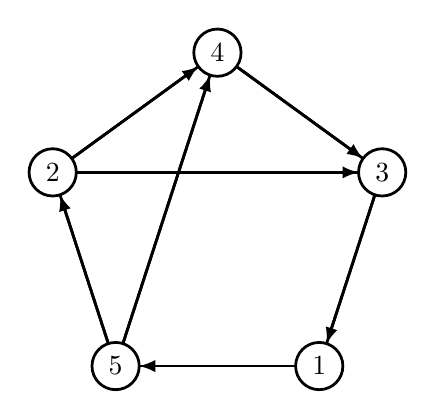
\begin{tikzpicture}[>=latex]

\def\r{2.2}
\coordinate (A) at ({\r*cos(-54+0*72)},{\r*sin(-54+0*72)});
\coordinate (C) at ({\r*cos(-54+1*72)},{\r*sin(-54+1*72)});
\coordinate (D) at ({\r*cos(-54+2*72)},{\r*sin(-54+2*72)});
\coordinate (B) at ({\r*cos(-54+3*72)},{\r*sin(-54+3*72)});
\coordinate (E) at ({\r*cos(-54+4*72)},{\r*sin(-54+4*72)});

\kante{(A)}{(E)}{1}
\kante{(B)}{(C)}{2}
\kante{(B)}{(D)}{13}
\kante{(C)}{(A)}{3}
\kante{(D)}{(C)}{6}
\kante{(E)}{(B)}{5}
\kante{(E)}{(D)}{6}

\knoten{(A)}{1}
\knoten{(B)}{2}
\knoten{(C)}{3}
\knoten{(D)}{4}
\knoten{(E)}{5}

\end{tikzpicture}
\end{center}
\end{column}
\begin{column}{0.59\hsize}

\only<1>{
\begin{block}{Pfade der Länge 1}
\[
A=
\begin{pmatrix}
0&0&1&0&0\\
0&0&0&0&1\\
0&1&0&1&0\\
0&1&0&0&1\\
1&0&0&0&0
\end{pmatrix}
\]
\end{block}
}

\only<2>{
\begin{block}{Pfade der Länge 2}
\[
A^2=\begin{pmatrix}
   0 & 1 & 0 & 1 & 0 \\
   1 & 0 & 0 & 0 & 0 \\
   0 & 1 & 0 & 0 & 2 \\
   1 & 0 & 0 & 0 & 1 \\
   0 & 0 & 1 & 0 & 0
\end{pmatrix}
\]
\end{block}
}

\only<3>{
\begin{block}{Pfade der Länge 3}
\[
A^3=\begin{pmatrix}
   0 & 1 & 0 & 0 & 2 \\
   0 & 0 & 1%
\begin{picture}(0,0)
\color{red}\put(-3,4){\circle{12}}
\end{picture}%
& 0 & 0 \\
   2 & 0 & 0 & 0 & 1 \\
   1 & 0 & 1 & 0 & 0 \\
   0 & 1 & 0 & 1 & 0
\end{pmatrix}
\]
\end{block}
}

\only<4>{
\begin{block}{Pfade der Länge 4}
\[
A^4=\begin{pmatrix}
   2%
\begin{picture}(0,0)
\color{red}\put(-3,4){\circle{12}}
\end{picture}%
& 0 & 0 & 0 & 1 \\
   0 & 1%
\begin{picture}(0,0)
\color{red}\put(-3,4){\circle{12}}
\end{picture}%
& 0 & 1 & 0 \\
   1 & 0 & 2%
\begin{picture}(0,0)
\color{red}\put(-3,4){\circle{12}}
\end{picture}%
& 0 & 0 \\
   0 & 1 & 1 & 1%
\begin{picture}(0,0)
\color{red}\put(-3,4){\circle{12}}
\end{picture}%
& 0 \\
   0 & 1 & 0 & 0 & 2%
\begin{picture}(0,0)
\color{red}\put(-3,4){\circle{12}}
\end{picture}%
\end{pmatrix}
\]
\end{block}
}

\only<5>{
\begin{block}{Pfade der Länge 5}
\[
A^5=\begin{pmatrix}
   1 & 0 & 2 & 0 & 0 \\
   0 & 1 & 0 & 0 & 2 \\
   0 & 2 & 1 & 2 & 0 \\
   0 & 2 & 0 & 1 & 2 \\
   2 & 0 & 0 & 0 & 1
\end{pmatrix}
\]
\end{block}
}

\only<6>{
\begin{block}{Pfade der Länge 6}
\[
A^6=\begin{pmatrix}
   0%
\begin{picture}(0,0)
\color{red}\put(-3,4){\circle{12}}
\end{picture}%
& 2 & 1 & 2 & 0 \\
   2 & 0%
\begin{picture}(0,0)
\color{red}\put(-3,4){\circle{12}}
\end{picture}%
& 0 & 0 & 1 \\
   0 & 3 & 0%
\begin{picture}(0,0)
\color{red}\put(-3,4){\circle{12}}
\end{picture}%
& 1 & 4 \\
   2 & 1 & 0 & 0%
\begin{picture}(0,0)
\color{red}\put(-3,4){\circle{12}}
\end{picture}%
& 3 \\
   1 & 0 & 2 & 0 & 0%
\begin{picture}(0,0)
\color{red}\put(-3,4){\circle{12}}
\end{picture}%
\end{pmatrix}
\]
\end{block}
}

\only<7>{
\begin{block}{Pfade der Länge 7}
\[
A^7=\begin{pmatrix}
   0%
\begin{picture}(0,0)
\color{red}\put(-3,4){\circle{12}}
\end{picture}%
& 3 & 0 & 1 & 4 \\
   1 & 0%
\begin{picture}(0,0)
\color{red}\put(-3,4){\circle{12}}
\end{picture}%
& 2 & 0 & 0 \\
   4 & 1 & 0%
\begin{picture}(0,0)
\color{red}\put(-3,4){\circle{12}}
\end{picture}%
& 0 & 4 \\
   3 & 0 & 2 & 0%
\begin{picture}(0,0)
\color{red}\put(-3,4){\circle{12}}
\end{picture}%
& 1 \\
   0 & 2 & 1 & 2 & 0%
\begin{picture}(0,0)
\color{red}\put(-3,4){\circle{12}}
\end{picture}%
\end{pmatrix}
\]
\end{block}
}

\only<8>{
\begin{block}{Pfade der Länge 8}
\[
A^8=\begin{pmatrix}
   4 & 1 & 0 & 0 & 4 \\
   0 & 2 & 1 & 2 & 0 \\
   4 & 0 & 4 & 0 & 1 \\
   1 & 2 & 3 & 2 & 0 \\
   0 & 3 & 0 & 1 & 4
\end{pmatrix}
\]
\end{block}
}

\only<9>{
\begin{block}{Pfade der Länge 9}
\[
A^9=\begin{pmatrix}
   4 & 0 & 4 & 0 & 1 \\
   0 & 3 & 0 & 1 & 4 \\
   1 & 4 & 4 & 4 & 0 \\
   0 & 5 & 1 & 3 & 4 \\
   4 & 1 & 0 & 0 & 4
\end{pmatrix}
\]
\end{block}
}

\only<10>{
\begin{block}{Pfade der Länge 10}
\[
A^{10}=\begin{pmatrix}
   1%
\begin{picture}(0,0)
\color{red}\put(-3,4){\circle{12}}
\end{picture}%
& 4 & 4 & 4 & 0 \\
   4 & 1%
\begin{picture}(0,0)
\color{red}\put(-3,4){\circle{12}}
\end{picture}%
& 0 & 0 & 4 \\
   0 & 8 & 1%
\begin{picture}(0,0)
\color{red}\put(-3,4){\circle{12}}
\end{picture}%
& 4 & 8 \\
   4 & 4 & 0 & 1%
\begin{picture}(0,0)
\color{red}\put(-3,4){\circle{12}}
\end{picture}%
& 8 \\
   4 & 0 & 4 & 0 & 1%
\begin{picture}(0,0)
\color{red}\put(-3,4){\circle{12}}
\end{picture}%
\end{pmatrix}
\]
\end{block}
}

\only<11>{
\begin{block}{Pfade der Länge 15}
\[
A^{15}=\begin{pmatrix}
    1 & 20 &  6 & 12 & 16 \\
   12 &  1 &  8 &  0%
\begin{picture}(0,0)
\color{red}\put(-3,4){\circle{12}}
\end{picture}%
&  6 \\
   16 & 18 &  1 &  6 & 32 \\
   20 &  6 &  8 &  1 & 18 \\
    6 &  8 & 12 &  8 &  1
\end{pmatrix}
\]
\end{block}
}

\only<12>{
\begin{block}{Pfade der Länge 20}
\[
A^{20}=\begin{pmatrix}
   33 & 56 &  8 & 24 & 80 \\
   24 & 17 & 32 & 16 &  8 \\
   80 & 32 & 33 &  8 & 80 \\
   56 & 24 & 48 & 17 & 32 \\
    8 & 48 & 24 & 32 & 33
\end{pmatrix}
\]
\end{block}
}

\only<13>{
\begin{block}{Pfade der Länge 25}
\[
A^{25}=\begin{pmatrix}
   193 & 120 &  74 &  40 & 240 \\
    40 & 113 &  80 &  80 &  74 \\
   240 & 114 & 193 &  74 & 160 \\
   120 & 154 & 160 & 113 & 114 \\
    74 & 160 &  40 &  80 & 193
\end{pmatrix}
\]
\end{block}
}

\only<14>{
\begin{block}{Pfade der Länge 30}
\[
A^{30}=\begin{pmatrix}
   673 & 348 & 460 & 188 & 560 \\
   188 & 433 & 160 & 240 & 460 \\
   560 & 648 & 673 & 460 & 536 \\
   348 & 700 & 400 & 433 & 648 \\
   460 & 400 & 188 & 160 & 673
\end{pmatrix}
\]
\end{block}
}

\only<15>{
\begin{block}{Pfade der Länge 35}
\[
A^{35}=\begin{pmatrix}
   1793%
\color{red}\drawline(-23,-3)(-23,10)(2,10)(2,-3)(-23,-3)
& 1644 & 1806 & 1108 & 1632 \\
   1108 & 1233 &  536 &  560 & 1806 \\
   1632 & 2914 & 1793%
\color{red}\drawline(-23,-3)(-23,10)(2,10)(2,-3)(-23,-3)
& 1806 & 2752 \\
   1644 & 2366 & 1096 & 1233 & 2914 \\
   1806 & 1096 & 1108 &  536 & 1793%
\color{red}\drawline(-23,-3)(-23,10)(2,10)(2,-3)(-23,-3)
\end{pmatrix}
\]
\end{block}
}

\end{column}
\end{columns}
\vbox to2cm{
\vfill
\only<3>{
	\begin{block}{Kürzester Verbindung von 3 nach 2}
	Der Weg 3---1---6---2 ist die kürzeste Verbindung von 3 nach 2
	\end{block}
}
\only<4>{
	\begin{block}{Kürzeste Zyklen}
	Jeder Knoten liegt auf einem Zyklus der Länge 4,
	dies sind die kürzesten Zyklen.
	1, 3 und 5 liegen auf beiden Zyklen, 2 und 4 nur auf einem.
	\end{block}
}
\only<6>{
	\begin{block}{Zyklen der Länge 6}
	{\em Keine} Zyklen der Länge 6
	\end{block}
}
\only<7>{
	\begin{block}{Zyklen der Länge 7}
	{\em Keine} Zyklen der Länge 7
	\end{block}
}
\only<10>{
	\begin{block}{Zyklen der Länge 10}
	Genau ein Zyklus der Länge 10
	\end{block}
}
\only<11>{
	\begin{block}{Verbindung von 4 nach 2}
	{\em Keine} Verbindung der Länge 15 von 4 nach 2
	\end{block}
}
\only<15>{
	\begin{block}{Zyklen der Länge 35}
	Es gibt 1793 Zyklen, die 1 enthalten, und sie enthalten alle auch 3 und 5
	\end{block}
}
}
\end{frame}
\egroup
